\documentclass[aps,twocolumn,secnumarabic,nobalancelastpage,amsmath,amssymb,
nofootinbib,superscriptaddress]{revtex4-1}


\usepackage{graphics}           % standard graphics specifications
\usepackage{graphicx}           % alternative graphics specifications
\usepackage{longtable}          % helps with long table options
\usepackage{url}                % for on-line citations
\usepackage{bm}                 % special 'bold-math' package
\usepackage[ngerman]{babel}     % deutsche Siblentrennung
\usepackage[utf8]{inputenc}     % Umlaute
\usepackage{upgreek}            % aufrechte (nicht-kursive) griech. Buchstaben
\usepackage[ngerman]{cleveref}  % abgekürzte Referenzen

\def\andname{\hspace*{-0.5em},} % definiert die Trennung zwischen 2 Autoren neu

\makeatletter
\setlength{\@fptop}{0pt}
\makeatother

% Titelseite
\begin{document}
\title{Compton-Effekt}
\author         {Ch. Egerland}
\email[Email: ]{egerlanc@physik.hu-berlin.de}
\author         {M. Pfeifer}

\email[Email: ]{max.pfeifer@physik.hu-berlin.de}
\affiliation    {Humboldt-Universität zu Berlin, Institut für Physik}
\date[Versuchsdatum: ]{13.06.2017}

%%%%%%%%%%%%%%%%%%%%%%%%%%%%%%%%%%%%%%%%%%%%%%%%%%%%%%%%%%%%%%%%%%%%%%%%%%%%%%%%
\begin{abstract}
  \noindent Gegenstand des Versuches ist die Untersuchung der Compton-Streuung von \textsuperscript{137}Cs-Photonen an einem Aluminium-Streutarget.
  Dazu werden die Spektren von drei Gammastrahlern (\textsuperscript{133}Ba, \textsuperscript{22}Na, \textsuperscript{137}Cs), sowie das Hintergrundrauschen
  mithilfe eines Szintillator-basierten Detektors aufgenommen. Die Spektren werden analysiert und aus den Messdaten wird das Auflösungsvermögen der Apparatur bestimmt.
  Außerdem erfolgt eine Berechnung des totalen Wirkungsquerschnittes für \textsuperscript{137}Cs .
\end{abstract}


\maketitle


%%%%%%%%%%%%%%%%%%%%%%%%%%%%%%%%%%%%%%%%%%%%%%%%%%%%%%%%%%%%%%%%%%%%%%%%%%%%%%%%

\section{Zur Theorie des Compton-Effektes}
Der Compton-Effekt ist ein Phänomen, welches bei der Streuung von Photonen an
Teilchen beobachtet wird. Hierbei gibt das Photon einen Teil seiner Energie an das
ruhende Teilchen ab, wodurch die Wellenlänge des Photons steigt und das Teilchen
sich bewegt. Dieser Mechanismus ist in Abbildung~\cref{fig:kinematik} veranschaulicht.
Die Energie des gestreuten $\gamma$-Quants ist gegeben durch:

  \begin{equation}
    E^* = \frac{E_0}{1+\gamma(1- cos \theta)}
    \label{eq:streuenergie}
  \end{equation}

Hierbei ist $\theta$ der Streuwinkel und $\gamma = E_0/mc^2$ das Verhältnis der
Energie des eintreffenden Photons zur Ruheenergie des Elektrons. Man sieht, dass
dieser Effekt sich erst für hohe Photonenergien (also $\gamma >> 1$) bemerkbar
macht.

\begin{figure}[h]
  \centering
  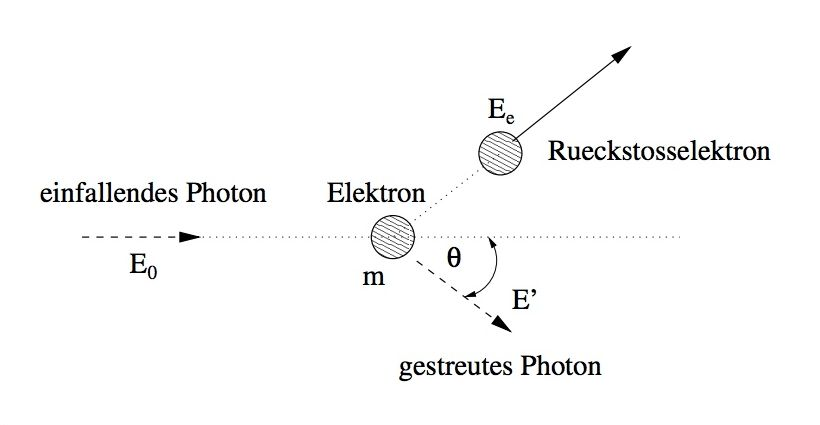
\includegraphics[width=0.5\textwidth]{comptstreu_schema.jpg}
  \caption{\label{fig:kinematik} Kinematik des Compton-Effekts aus \cite{skript07}.}
\end{figure}

Der korrekte differentielle Wirkungsquerschnitt, der die Winkelverteilung des
Compton-Effektes beschreibt, ist durch die Klein-Nishina-Formel gegeben:

  \begin{equation}
    \frac{d \sigma}{d \Omega} = \frac{r_0^2}{2} \left( \frac{E^*}{E_0} \right)^2
    \left( \frac{E_0}{E^*} + \frac{E^*}{E_0} - sin^2 \theta    \right)
    \label{eq:kleinnishina}
  \end{equation}

Aus dieser Formel folgt, dass es eine Vorwärts-Rückwärts-Asymmetrie gibt, d.h.
es werden mehr Photonen in die Vorwärtsrichtung, als in die Rückwärtsrichtung
gestreut.


%%%%%%%%%%%%%%%%%%%%%%%%%%%%%%%%%%%%%%%%%%%%%%%%%%%%%%%%%%%%%%%%%%%%%%%%%%%%%%%%
\section{Experiment}
Der Versuchsaufbau ist in Abbildung ~\cref{fig:aufbau} gezeigt. Die Photonen treten
aus der Strahlungsquelle (Daten in Tabelle ~\cref{tab:materialien}) in den Kolliminator
welcher dafür sorgt, dass die Photonen aus nahezu 0 Grad kommen. Das Aluminium-
Streutarget ist herausnehmbar.

\begin{figure}[h]
  \centering
  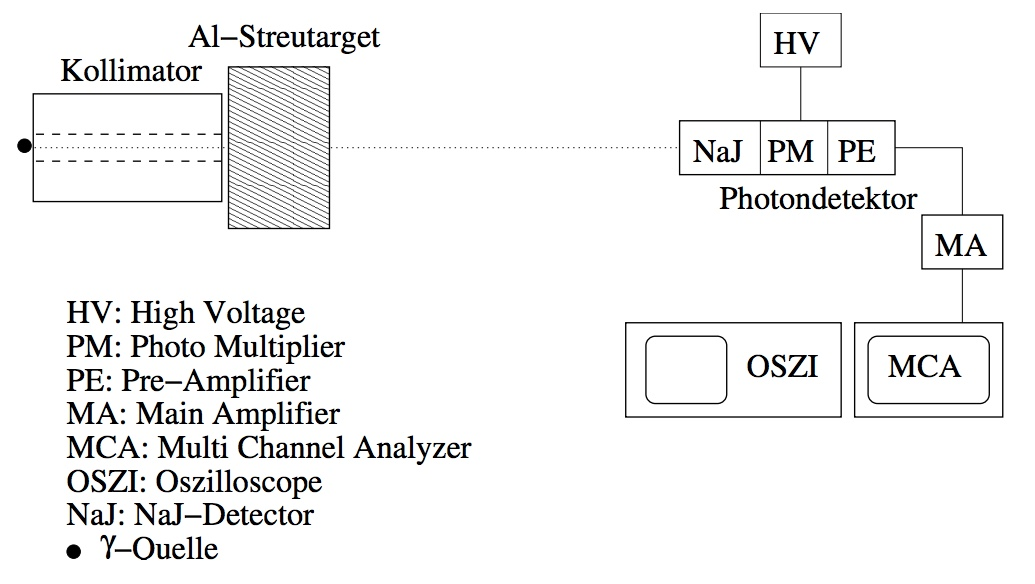
\includegraphics[width=0.5\textwidth]{aufbau.jpeg}
  \caption{\label{fig:aufbau} Versuchsaufbau aus \cite{skript07}.}
\end{figure}

Die Photonen treffen auf den Detektor, der in unserem
Fall aus einem mit Thallium dotierten NaI-Szintillator besteht. Ein eintreffendes Photon
erzeugt im NaI-Kristall ein Elektron-Loch-Paar welches sich zum Aktivatorzentrum
(Thallium) bewegt und dieses anregt. Durch Emission von Licht kehrt das Thallium
nun wieder in seinen Grundzustand zurück. Die aus dem Detektor gelösten Photonen
werden nun im Photomultiplier verstärkt. Hierbei trifft ein Photon auf den
Photomultiplier und löst durch den Photoeffekt ein Elektron, welches im weiteren
Verlauf weitere Elektronen aus den Dynoden herausschlägt (die sogenannten
Sekundärelektronen). Somit entsteht eine Spannung, welche wir als proportional zur
Energie der am Szintillator eintreffenden Photonen betrachten können. Diese
Spannung wird durch zwei OP Amplifier verstärkt und gelangt nun in den Multi

\begin{table}[h]
\begin{ruledtabular}
\begin{tabular}{cccc}
 Präparat & $\gamma$-Energie in MeV & Aktivität (kBq) & Halbwertszeit\\
\hline
^{133} Ba & 0.356 & 397 & 10.54a \\
^{22} Na & 0.511 & 374 & 2.603a \\
^{137} Cs & 0.662 & 371 & 30.17a \\
\end{tabular}
\end{ruledtabular}
\caption{\label{tab:materialien} Daten der Photonenquellen ermittelt am 01.11.1996
mit einem Fehler von 4\%.}
\end{table}

Channel Analyzer, welcher dafür sorgt, dass die eintreffenden Impulse mit verschiedener
Amplitude entsprechend diese einem Kanal zugeordnet werden. Diese Kanäle können
wir am PC auslesen und in einem Histogramm darstellen, wir sehen also ein Diagramm,
dass uns die Counts in den jeweiligen Kanälen zeigt. Daraus lässt sich mithilfe einer Kalibrationskurve,
die den Kanälen eine Energie zuordnet, das Energiespektrum bestimmen.

Zunächst ist es aus gesundheitlichen Erwägungen erforderlich, die Äquivalentdosis zu bestimmen, der man

\noindent während des Versuches ausgesetzt ist. Hierfür wird eine Experimentierdauer von 12 Stunden und eine
vollständige Absorption der Probenstrahlung angenommen. Die Äquivalentdosis H ist im Falle von Photonen
gleich der Dosis D \cite{qfaktor}. Die Dosisleistung ist definiert als

\begin{equation}
  \dot{D} = \frac{E_\gamma \cdot A}{m}
\end{equation}\vspace{0.5em}

\noindent mit der bestrahlten Masse $m$, der Aktivität $A$ der Photonenquelle und der Photonenenergie $E_\gamma$, wobei die Aktivität ein
zeitlich exponentiell abfallendes Verhalten zeigt:

\begin{equation}
  A(t)=A_0}\cdot exp\left( -\frac{t}{\tau}\right) =A_0\cdot exp\left(-\frac{t}{t_{1/2}}\cdot ln(2)\right)
\end{equation}\vspace{0.5em}

\noindent Dabei bezeichnet $A_0$ die Aktivität der Quelle am 01.11.1996 (s. Tabelle 1). Durch Integration der Dosisleistungen über die Zeit und Aufsummieren
der Dosisbeiträge der drei Proben gelangt man unter Annahme einer bestrahlten Masse von $m\approx 75$kg zu einer maximalen Äquivalentdosis von 17,5 $\upmu\text{Sv}$ (s. Anhang A1-A2).
Das entspricht einem Zuwachs der durchschnittlichen jährlichen Strahlungsbelastung ($\approx 2,1$ mSv \cite{jdosis}) um 0,8\%.

\vspace{1em}\noindent Da das Signal des Szintillators einen Vor- und Hauptverstärker durchläuft, ist die Messung einer Totzeit unterworfen. Das Messprogramm (MAESTRO)
quantifiziert diese Totzeit bereits und liefert Werte in der Größenordnung von 3 $\upmu\text{s}$ bis 17 $\upmu\text{s}$. Eine grafische, softwareunabhängige Abschätzung mit
dem Oszilloskop ergibt ähnliche Totzeiten in der Größenordnung von 8 $\upmu\text{s}$. Die Zeit, die der Detektor zur Messung eines Ereignisses benötigt, beträgt mit 6 ms drei
Größenordnungen mehr als die Totzeit, womit diese vernachlässigt werden kann. %HIER VLLT NOCH VGL WIE VIELE SIGNALE ABSOLUT VERLOREN GEGANGEN SIND

%%%%%%%%%%%%%%%%%%%%%%%%%%%%%%%%%%%%%%%%%%%%%%%%%%%%%%%%%%%%%%%%%%%%%%%%%%%%%%%%
\section{Daten und Analyse}
\subsection{Spektren}

\vspace{1em}\noindent Die ohne Streutarget aufgenommen Spektren der Gammastrahler sind in \cref{fig:spektrenK}: dargestellt. Da das Messprogramm die Ereignisse verschiedenen Kanälen (2048 Kanäle)
zuordnet, werden diese mithilfe einer Kalibrationskurve K(E) in Energien umgesetzt. Dazu wurden die charakteristischen Peaks der Spektren mit MATLAB einem Gauß-Fit unterzogen, der
die genauen Peakpositionen einschließlich deren Unsicherheit liefert. Aufgrund der unterschiedlichen Messzeiten der Spektren (insb. Rauschen) und zwecks Vergleich wurden die
Funktionswerte der Energiespektren (Ereignisse) auf die jeweiligen Offenzeiten normiert. Außerdem wurde das (normierte) Rauschsignal von allen Spektren abgezogen,
sodass diese bereits korrigiert sind.

Die Fits liefern folgende Parameter:

\begin{table}[h]
\begin{ruledtabular}
\begin{tabular}{cccc}
 Spektrum & Peak-Position (Kanal) & Gaußbreite $\sigma\text{ (keV)}$ \\
\hline
^{133} Ba & 265,7\:\pm\: 0,5 & 91 \\
^{22} Na & 397,52\:\pm\: 0,28\:\cite{NaK} & 14\:\cite{NaK} \\
^{137} Cs & 523,0\:\pm\: 0,30 & 99 \\
\end{tabular}
\end{ruledtabular}
\caption{\label{tab:peakssigma} Peakbreiten der Gauß-Fits }
\end{table}


Wie in \cref{fig:spektrenK1} zu erkennen, zeigt die Messung des $^{22}\text{Na}$ kein ausgeprägtes, charakteristisches Maximum. Hier liegt schlicht ein Experimentierfehler vor.
Da Natrium eine geringe Aktivität hat, sollte die Probe sinnvollerweise näher an den Detektor gerückt werden, da sonst in kurzer Zeit zu wenig Ereignisse stattfinden. Dies
wurde leider nicht berücksichtigt. Daher wird zur Erstellung der Kalibrationskurve der in \cref{tab:peakssigma} angegebene Messwert verwendet:
\begin{figure}[h]
  \centering
  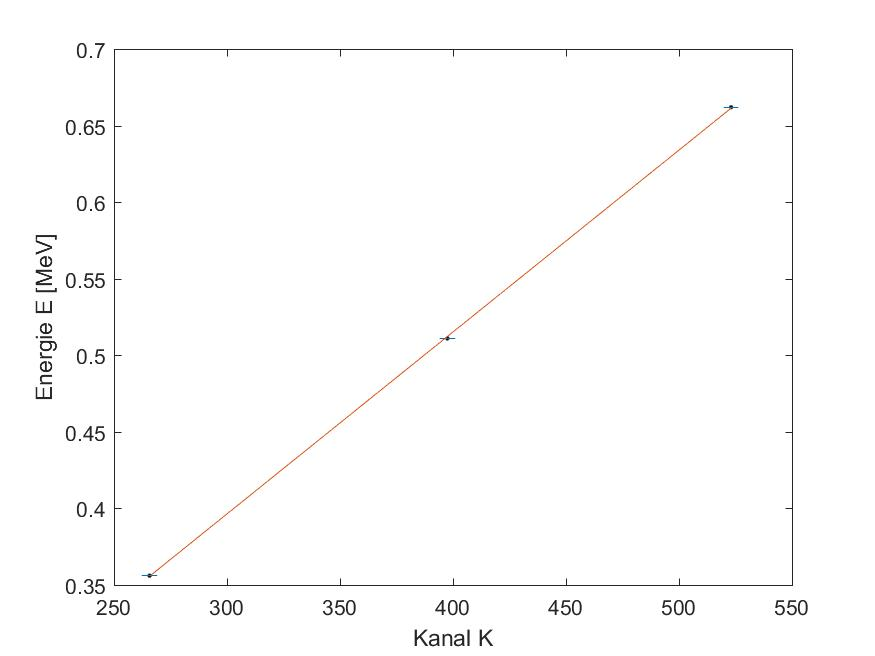
\includegraphics[width=0.5\textwidth]{../Messung/eichkurveEvonK.jpg}
  \caption{\label{fig:EvonK} lineare Eichkurve E(K) des Messsystems}
\end{figure}

\newpage
\subsection{Auflösung}
\noindent Aus den Halbwertsbreiten $\text{FWHM}=2.35\sigma(E)$ lässt sich nun die Auflösungfunktion aufstellen:
\begin{equation*}
    A(E) = \frac{\sigma(E)}{E}
\end{equation*}

\noindent Da die Energiewerte, genau wie die Anzahl der Ereignisse, unabhängig voneinander auftreten und beide Größen proportional zueinander sind, folgt, dass für die
Gaußbreite der Energiewerte $\sigma(E)\propto\sqrt{E}$ gilt. Die Auflösung wird mit zunehmender Enenergie also immer besser, genauer:
\begin{equation*}
    A(E) \propto \frac{1}{\sqrt{E}}
\end{equation*}
\begin{figure}[h]
  \centering
  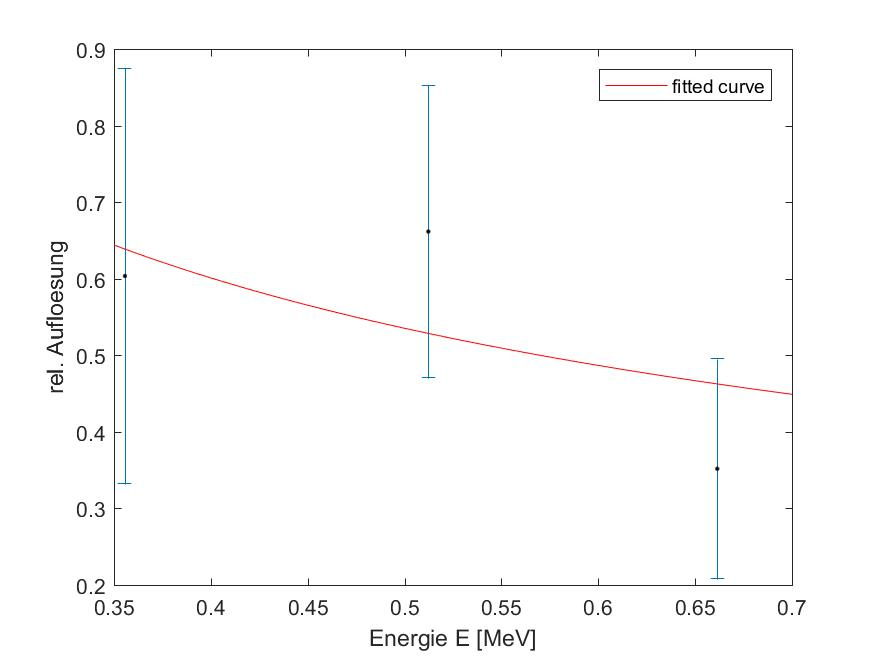
\includegraphics[width=0.5\textwidth]{../Messung/relAufl.jpg}
  \caption{\label{fig:relAufl} relative Auflösung des Detektors in Abhängigkeit von der Photonenenergie}
\end{figure}

\noindent Der Fit ergibt folgende Auflösungen für die verschiedenen Präparate (Parameter $a\approx 0.39$, $b\approx -0.02$):

\begin{equation}
  \begin{gathered}
    A_{Ba} = 0,64   \\
    A_{Cs} = 0,46   \\
    A_{Na} = 0,53
    \caption{\label{eq:aufloe}}
  \end{gathered}
\end{equation}

\vspace{1em}\noindent Das Energiespektrum von $^{137}Cs$ ist in \cref{fig:CsUnkK} (Anhang) unkorrigiert und um das Rauschsignal korrigiert dargestellt. Drei Abschnitte sind
qualitativ eindeutig einzuordnen:
Der Gaußpeak bei 0,66 MeV ist der Photopeak. Hier gibt das beim Zerfall $^{137}Cs\rightarrow {^{137}Ba}^*\rightarrow {^{137}Ba} \: + \: \gamma$ entstehende Photon seine
gesamte Energie unter Erzeugung eines Elektron-Loch-Paares an den NaI-Kristall ab.
Findet Comptonstreuung statt, erfährt das Photon nach \cref{eq:streuenergie} eine maximale energetische Abschwächung bei $\theta=\pi$ auf
$E_{\gamma,min}=E^*=0,18$ MeV. Das Elektron erhält die Differenzenergie von
\begin{equation*}
  E_e=0,66\text{ MeV} - 0.18\text{ MeV} = 0,48\text{ MeV}
\end{equation*}
die es dann im Szintillator abgibt. Diese maximale Elektronenenergie
bezeichnet man als Compton-Kante, deren theoretische Lage in guter Übereinstimmung mit \cref{fig:CsUnkK} ist.
Events, die unterhalb von 480 keV registriert sind, entstammen ebenfalls der Compton-Streuung an Elektronen bei kleineren Ablenkwinkeln. Das sog. Compton-Kontinuum
ist in der Abb. gut erkennbar.
Auffällig sind außerdem die Counts im Bereich zwischen 0.1 MeV und 0.3 MeV. Der Peak bei 0.2 MeV wird durch Photonen verursacht, die bei $\theta=\pi$ außerhalb des
Detektors gestreut wurden und dann ihre Energie im Szintillator deponieren. Erfährt das Photon Mehrfachstreuung, desto weniger Energie wird im Szintillator registriert,
womit sich die Ereignisse zwischen 0.1 MeV und 0.2 MeV erklären lassen (je mehr Wechselwirkungen, desto geringer die Wahrscheinlichkeit den Detektor zu treffen $\rightarrow$ Abnahme der Counts).

\begin{figure*}[h]
  \begin{minipage}[t]{0.49\textwidth}
    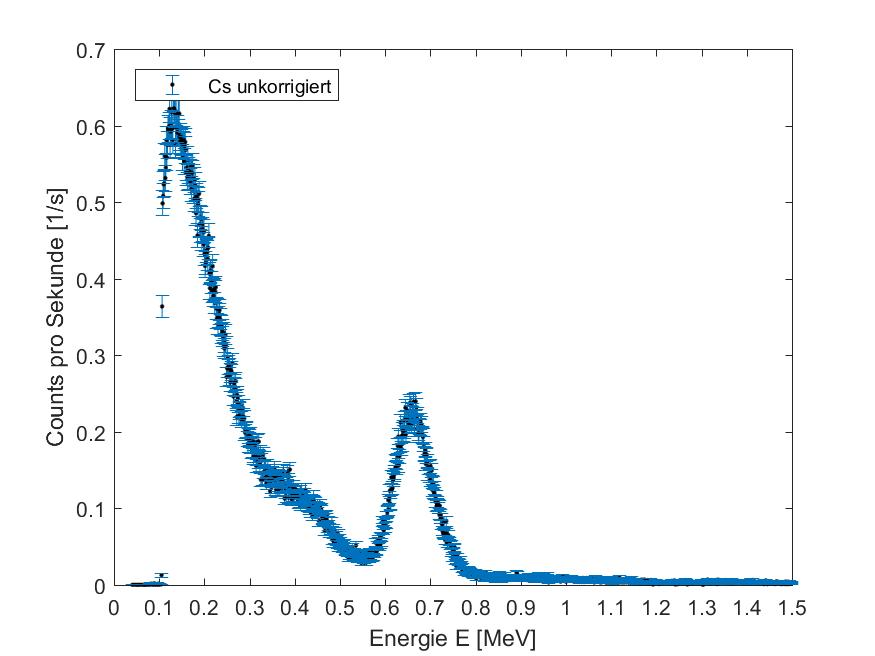
\includegraphics[width=\textwidth]{../Messung/Csuk.jpg}
  \end{minipage}
  \begin{minipage}[t]{0.49\textwidth}
    \includegraphics[width=\textwidth]{../Messung/Csk.jpg}
  \end{minipage}
  \caption{\label{fig:CsUnkK} links unkorrigiertes, rechts um Rauschen korrigiertes Energiespektrum von $^{137}Cs$}
\end{figure*}

\vspace{0.5em}\noindent Wäre die Gaußbreite $\sigma(E)=0$ würde der Photopeak wie in \cref{fig:deltaspek} (Anhang) einer Deltafunktion entsprechen. Die natürliche Linienbreite
lässt sich mithilfe der Heisenberg'schen Unschärferelation berechnen:
\begin{equation*}
    \Delta E \Delta t \geq \frac{\hbar}{2}
\end{equation*}
Wird $t$ durch die Lebensdauer $t_{Ba}=2,5\text{ min}$ \cite{skript07} des angeregten Zustands von $^{137}Ba$ angenähert gelangt man zu einer natürlichen Linienbreite von
\begin{equation}
    \Delta E=2,2\cdot10^{-18}\text{ eV}
    \caption{\label{eq:natLin}}
\end{equation}
wodurch eine maximale Auflösung von
\begin{equation}
    \frac{\Delta E}{E}=3,3\cdot10^{-14}\text{ eV}
\end{equation}
erreichbar wäre. Verglichen mit der erreichten Auflösung in der Größenordnung von $10^{-1}$ ist die nur durch die natürliche Linienbreite bedingte Auflösung verschwindend klein.
Ein weiterer Einfluss, der zu einer Linienverbreiterung führt ist, dass die Elektronen im Atom bereits eine kinetische Energie besitzen. Dieser Störfaktor lässt sich quantifizieren,
indem die durchschnittliche kinetische Energie eines Elektrons in einem Atom mit Kernladungszahl $Z$ berechnet wird:
\begin{equation*}
  \begin{gathered}B
    F_C=F_{rad} \Longleftrightarrow E_{e,kin}=\frac{1}{8\pi \epsilon_0}\frac{Z\cdot e^2}{r} \\
    E_{e,kin} = \Delta E = 73,5\text{ eV}
  \end{gathered}
\end{equation*}
Dabei wurde der Abstand $r$ des Elektrons vom Kern als der Bohr'sche Radius $a_0\approx 5,3\cdot 10^{-11}\text{ m}$ genähert und eine Kernladungszahl $Z=54$
des als Spurenelement in der Luft vorkommenden Xenon-Kerns (möglichst hohe Kernladungszahl) angenommen.
Diese Korrektur ist im Vergleich zur natürlichen Linienbreite \cref{eq:natLin} wesentlich größer, jedoch resultiert daraus maximale Auflösung von
\begin{equation}
    \frac{\Delta E}{E}=1,1\cdot10^{-4}\text{ eV}
\end{equation}
welche ebenfalls vernachlässigbar klein gegen die berechnete Auflösung \cref{eq:aufloe} ist. Offenbar haben der statistische Fehler und die zeitliche Auflösung des Detektorsystems
den größten Einfluss auf die Linienbreite.

\subsection{Wirkungsquerschnitt}
Der totale Wirkungsquerschnitt für Compton-Streuung ist gegeben durch $\cite{skript07}$:
\begin{equation}
    WQ Formel
    \caption{\label{eq:totWQ}}
\end{equation}





%%%%%%%%%%%%%%%%%%%%%%%%%%%%%%%%%%%%%%%%%%%%%%%%%%%%%%%%%%%%%%%%%%%%%%%%%%%%%%%%

\section{Schlussfolgerung}

Schlussoflgerung, sollten wir mal was von nem Buch oder so entnehmen nutzen wir:


\begin{quote}
  Ein Zitat mit Referenz auf das Buch\cite{melissinos1966}
\end{quote}

Lorem ipsum dolor sit amet, consectetur adipiscing elit. Nam id facilisis ligula,
a ultrices nibh. Nullam suscipit tellus nec mauris fermentum, ornare luctus neque
tincidunt. Aenean commodo tincidunt varius. Phasellus faucibus metus non erat
consectetur bibendum. Duis et luctus risus, at egestas justo. Nunc eleifend lacus
ac laoreet scelerisque. Aenean cursus dignissim magna in ultrices. In eget nisl
quis nisi.


%%%%%%%%%%%%%%%%%%%%%%%%%%%%%%%%%%%%%%%%%%%%%%%%%%%%%%%%%%%%%%%%%%%%%%%%%%%%%%%%
\bibliography{sample-paper}
\bibliographystyle{prsty}
\begin{thebibliography}{99}
\bibitem{skript07}O.Epler, U. Schwanke, Compton-Effekt (Versuchsskript), [2007]
\bibitem{qfaktor}H.Krieger, Grundlagen der Strahlungsphysik und des Strahlenschutzes (S. 323), Springer Verlag, 4. Auflage [2004]
\bibitem{jdosis}Bundesamt für Strahlenschutz, "Wie hoch ist die natürliche Strahlenbelastung in Deutschland?\grqq\: (unter http://www.bfs.de/DE/themen/ion/umwelt/natuerliche-strahlenbelastung/natuerliche-strahlenbelastung_node.html)
\bibitem{NaK}Jan Beier, Paul Ledwon: Versuchsprotokoll Compton-Effekt, [2017]
\end{thebibliography}


%%%%%%%%%%%%%%%%%%%%%%%%%%%%%%%%%%%%%%%%%%%%%%%%%%%%%%%%%%%%%%%%%%%%%%%%%%%%%%%%
\clearpage
\appendix

\section{ }

% Strahlendosisberechnung
\begin{equation}
  D = \sum\limits_{i=1}^3 \int\limits_{t_1}^{t_2} \! \dot{D_i}(t) \, \mathrm{d}t = \frac{1}{m}\sum\limits_{i=1}^3
  \frac{1}{E_{\gamma,i}} \int\limits_{t_1}^{t_2} \! A_{i}(t) \, \mathrm{d}t  \newline
\end{equation}
mit $t_1 = 20,263a$ und $t_2 = 20,263a$ + 12h
\begin{equation}
  \begin{gathered}
    D_i = \cfrac{E_{\gamma,i}}{m} \int\limits_{t_1}^{t_2} \! A_i(t) \, \mathrm{d}t \\
    = \cfrac{E_{\gamma,i}\cdot A_{0,i}}{m} \int\limits_{t_1}^{t_2} \! exp\left(-\frac{t}{t_{1/2}}\cdot ln(2)\right) \, \mathrm{d}t
  \end{gathered}
\end{equation}
\Rightarrow D_{Ba} = 3.36\:$\upmu\text{Sv}$,\: D_{Na} = 0.07\:$\upmu\text{Sv}$,\: D_{Cs} = 14.11\:$\upmu\text{Sv}$
\vspace{3em}

\begin{figure}[h]
  \centering
  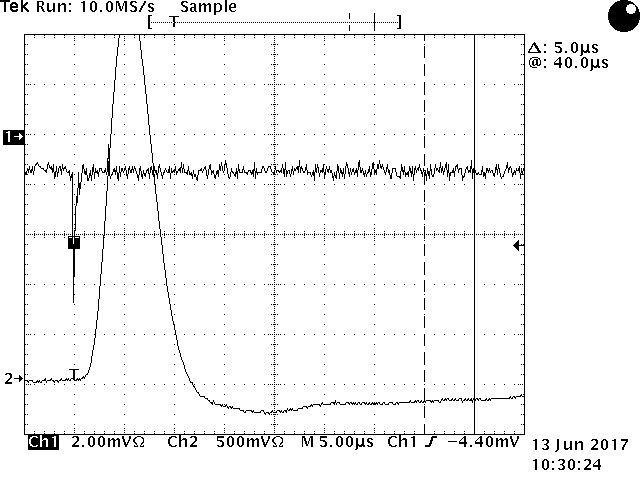
\includegraphics[width=0.5\textwidth]{../Messung/OsziVerstaerkerkurve/TEK00009.jpg}
  \caption{\label{fig:aufbau} Vor- und Hauptverstärkersignal Oszilloskop}
\end{figure}

\begin{figure}[h]
  \centering
  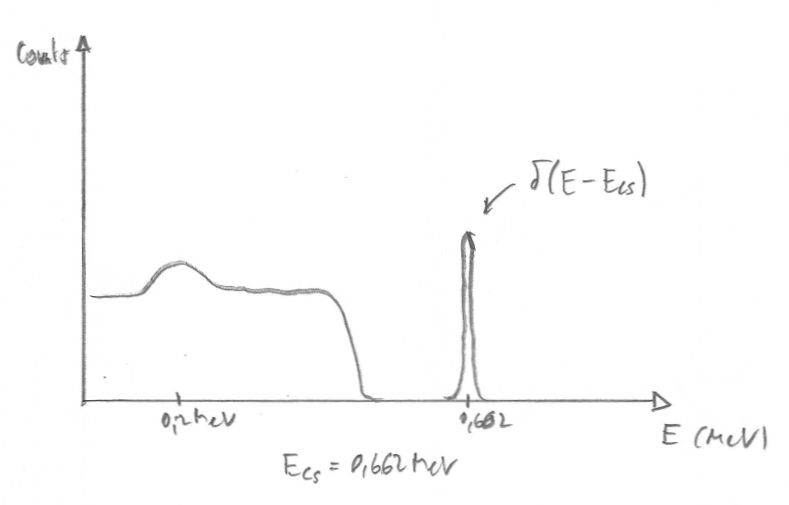
\includegraphics[width=0.5\textwidth]{../Messung/deltaspektrum.jpg}
  \caption{\label{fig:deltaspek} hypothetisches Energiespektrum von $^{137}Cs$ mit $\sigma(E)=0$}
\end{figure}


\begin{figure*}[b]
  \begin{minipage}[t]{0.49\textwidth}
    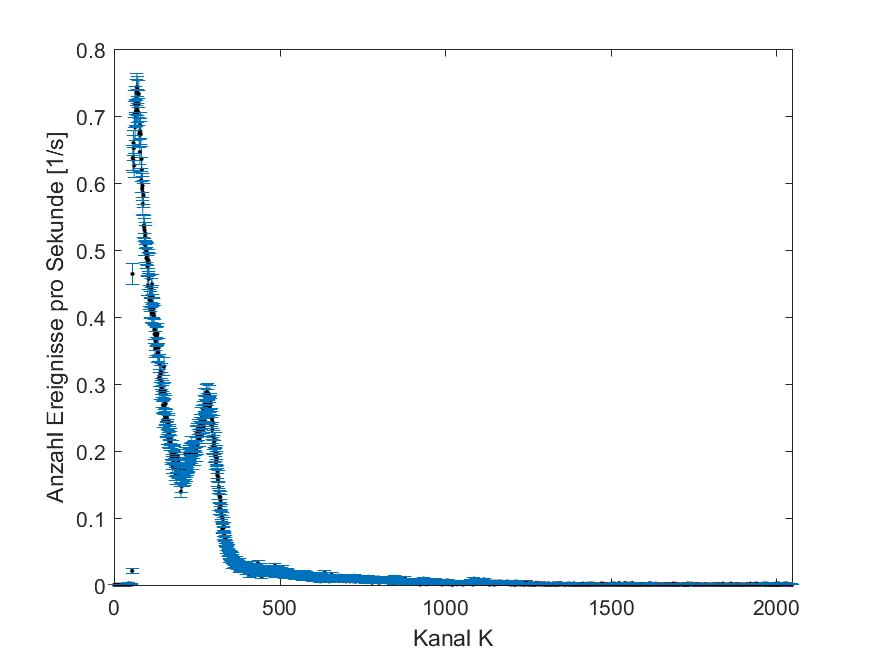
\includegraphics[width=\textwidth]{../Messung/BaK.jpg}
  \end{minipage}
  \begin{minipage}[t]{0.49\textwidth}
    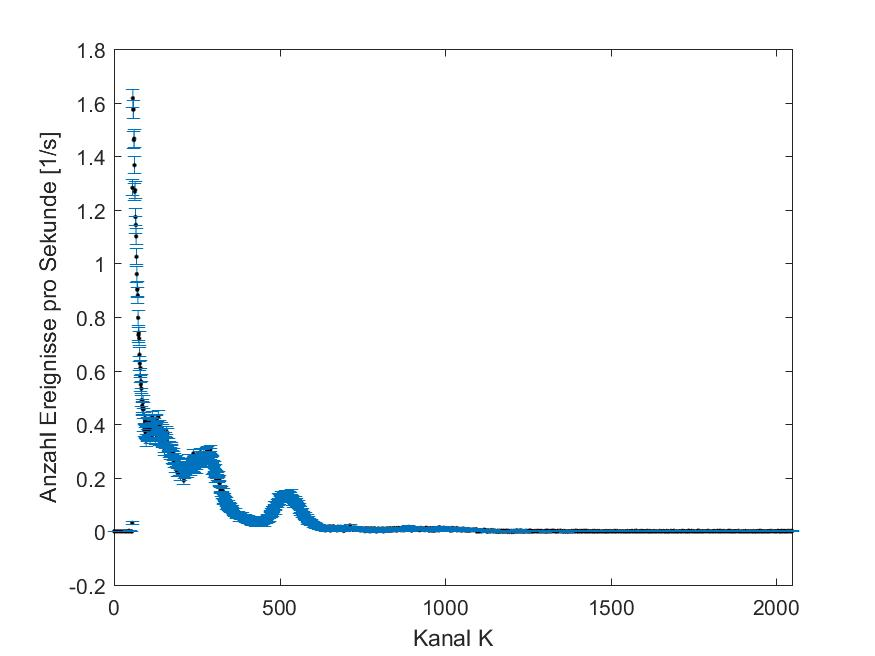
\includegraphics[width=\textwidth]{../Messung/NaK.jpg}
  \end{minipage}
  \caption{\label{fig:spektrenK1} korrigierte Spektren der Präparate (Ereignisse vs Kanal); links \textsuperscript{133}Ba, rechts \textsuperscript{22}Na}
\end{figure*}
\begin{figure*}[t]
  \begin{minipage}[t]{0.49\textwidth}
    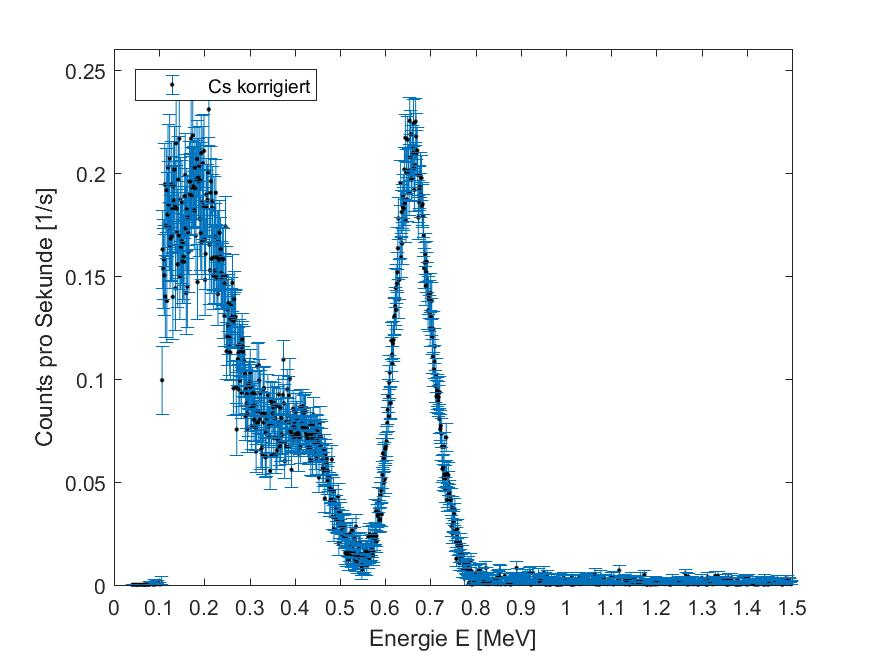
\includegraphics[width=\textwidth]{../Messung/CsK.jpg}
  \end{minipage}
  \begin{minipage}[t]{0.49\textwidth}
    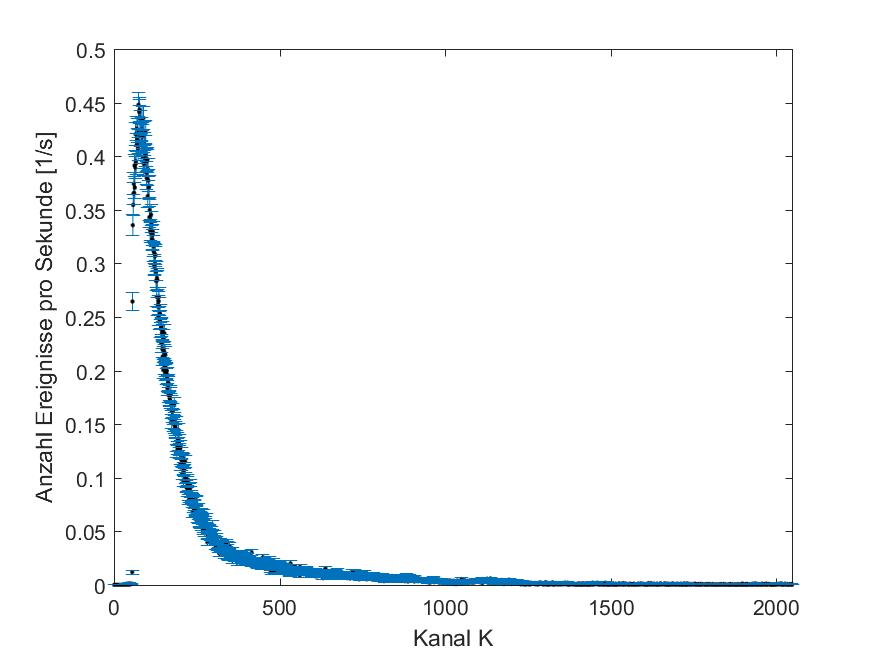
\includegraphics[width=\textwidth]{../Messung/Rauschen.jpg}
  \end{minipage}
  \caption{\label{fig:spektrenK2} korrigierte Spektren der Präparate (Ereignisse vs Kanal); links \textsuperscript{137}Cs, rechts Rauschen}
\end{figure*}

Hier sehen wir einen Beispiel Anhang und so könnte man Code in Latex einbinden:
\begin{verbatim}
> mkdir ~/8.13
> mkdir ~/8.13/papers
> mkdir ~/8.13/papers/template
> cd ~/8.13/papers/template
\end{verbatim}


%%%%%%%%%%%%%%%%%%%%%%%%%%%%%%%%%%%%%%%%%%%%%%%%%%%%%%%%%%%%%%%%%%%%%%%%%%%%%%%%


\end{document}
